\setcounter{chapter}{15}% Equivalent to "letter O"
\renewcommand{\thechapter}{\Alph{chapter}}
\Chapter{An�lisis de resultados}


\justify
\section{Clasificaci�n de las carreras tentativas}

\begin{table}[H]
	\begin{center}
		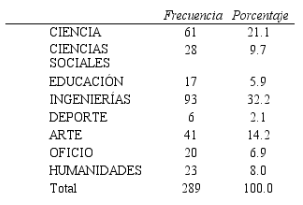
\includegraphics{clasificacionTentativas}
		\caption{Frecuencia y porcentaje de los estudiantes seg�n sus categor�as de carrera tentativa}
		\label{fig:clasificacionTentativas}
	\end{center}
\end{table}

	Se clasificaron las respuestas que los estudiantes ingresaron en la encuesta en 8 categor�as. De esta manera, se logra encontrar a qu� rama pertenecen las carreras tentativas que los estudiantes de la Universidad manifiestan como favoritas. Se logra observar que la categor�a que m�s sobresale es la ingenier�a y en segundo la categor�a ciencia. Muchos de estos ingenieros, si bien es cierto est�n cursando una carrera de esta �ndole, preferir�an estar en otro tipo de ingenier�a, pero muchos de ellos debido a factores externos se ven obligados a seguir otra ingenier�a. Por otra parte, algunos de ellos manifestaron estar a gusto con su carrera, sin embargo la carrera que cursan tiene relaci�n o servir� de conexi�n para llegar a la ingenier�a que realmente desean seguir. De igual manera, dicha respuesta aplica para ciencias puras, ya que algunos mencionan que su ingenier�a les sera de utilidad para cursar alguna carrera mas aplicada a lo cient�fico. Por �ltimo, las 3 facultades restantes est�n sus respuestas est�n dispersas en las categor�as restantes.\\


\section{Correlaci�n entre carreras tentativas y universitarias}

\begin{table}[H]
	\begin{center}
		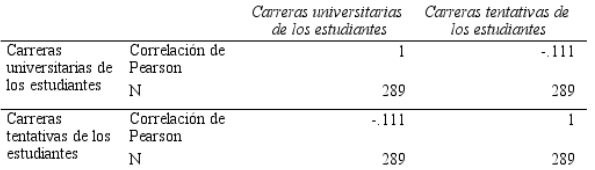
\includegraphics{correlacionTentativa}
		\caption{Correlaci�n entre la categor�a de las carreras tentativas y las universitarias de los estudiantes}
		\label{fig:correlacionTentativa}
	\end{center}
	\end{table}


\section{Estudiantes que encuentran una relaci�n entre carrera tentativa y universitaria}

\begin{figure}[H]
	\begin{center}
		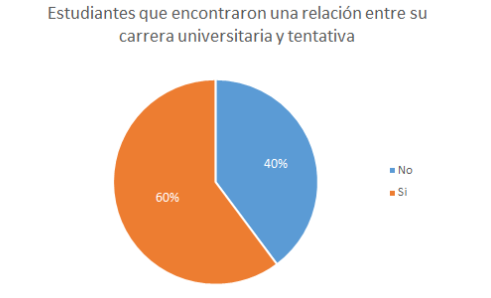
\includegraphics{encontraronRelacion}
		\caption{Estudiantes de la UVG que encontraron una relaci�n entre su carrera tentativa y universitaria}
		\label{fig:encontraronRelacion}
	\end{center}
\end{figure}


\section{Estudiantes que encuentran una relaci�n entre carrera tentativa y universitaria}

\begin{figure}[H]
	\begin{center}
		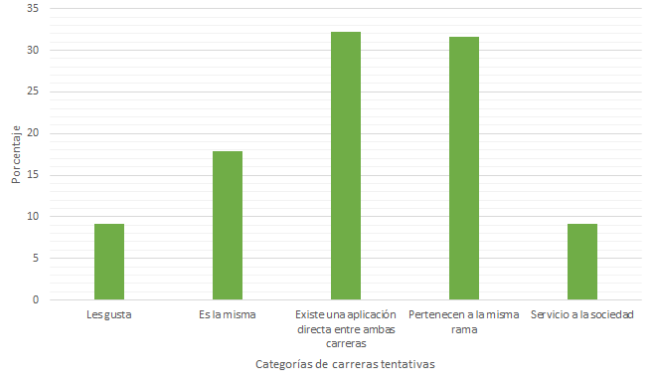
\includegraphics{categoriasRelaciones}
		\caption{Categorizaci�n de las relaciones entre la carrera tentativa y universitaria encontradas por los estudiantes}
		\label{fig:categoriasRelaciones}
	\end{center}
\end{figure}


\section{Satisfacci�n de los estudiantes con su carrera universitaria}

\begin{figure}[H]
	\begin{center}
		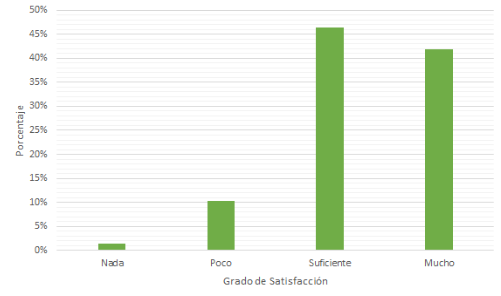
\includegraphics{gradoSatisfaccion}
		\caption{Grado de satisfacci�n de los estudiantes de la UVG con su carrera universitaria}
		\label{fig:gradoSatisfaccion}
	\end{center}
\end{figure}


\section{Estudiantes que escogieron su carrera tentativa como universitaria}

\begin{figure}[H]
	\begin{center}
		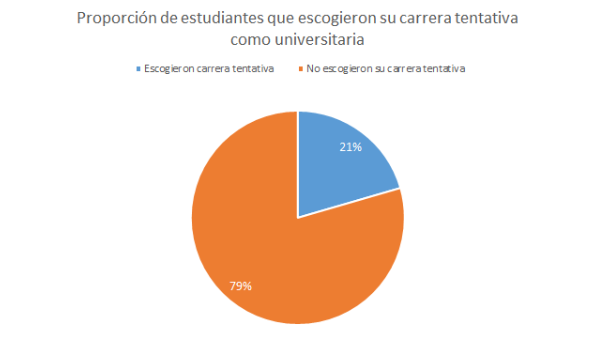
\includegraphics{tentativaUniversitaria}
		\caption{Proporci�n de los estudiantes que escogieron su carrera tentativa como universitaria}
		\label{fig:tentativaUniversitaria}
	\end{center}
\end{figure}

\begin{table}[H]
	\begin{center}
		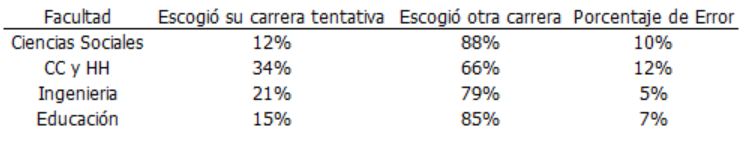
\includegraphics{tentativaUniversitariaFacultad}
		\caption{Porcentaje de estudiantes de la UVG que escogieron su carrera de etapa tentativa como universitaria seg�n su facultad}
		\label{fig:tentativaUniversitariaFacultad}
	\end{center}
\end{table}


\section{Influencia de ciertos factores en la elecci�n de carrera universitaria}

\begin{table}[H]
	\begin{center}
		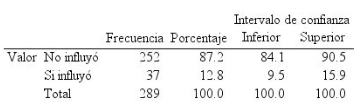
\includegraphics{factorPopularidad}
		\caption{Estudiantes que indicaron que el factor popularidad de la carrera los influenci�}
		\label{fig:factorPopularidad}
	\end{center}
\end{table}

\begin{table}[H]
	\begin{center}
		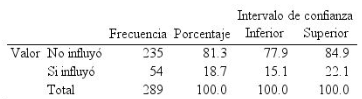
\includegraphics{factorPadres}
		\caption{Estudiantes que indicaron que el factor influencia de los padres o encargados los influenci�}
		\label{fig:factorPadres}
	\end{center}
\end{table}

\begin{table}[H]
	\begin{center}
		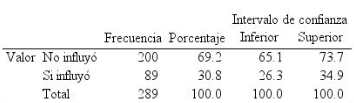
\includegraphics{factorRemuneracion}
		\caption{Estudiantes que indicaron que el factor remuneraci�n de la carrera los influenci�}
		\label{fig:factorRemuneracion}
	\end{center}
\end{table}

\begin{table}[H]
	\begin{center}
		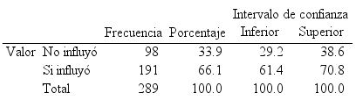
\includegraphics{factorOportunidad}
		\caption{Estudiantes que indicaron que el factor oportunidad laboral de la carrera los influenci�}
		\label{fig:factorOportunidad}
	\end{center}
\end{table}


\section{Distribuci�n de carreras tentativas seg�n el sexo del estudiante}

\begin{table}[H]
	\begin{center}
		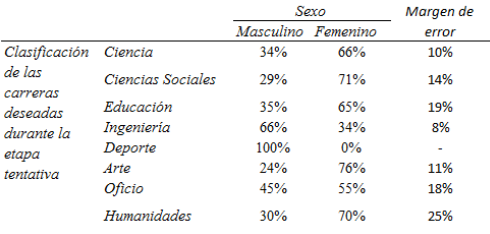
\includegraphics{SexoTentativa}
		\caption{Cuadro de contingencia entre sexo y categor�a de carrera tentativa del estudiante}
		\label{fig:SexoTentativa}
	\end{center}
\end{table}


\section{Correlaci�n entre influencia de los padres y posibilidad de elecci�n de carrera de los estudiantes}

\begin{table}[H]
	\begin{center}
		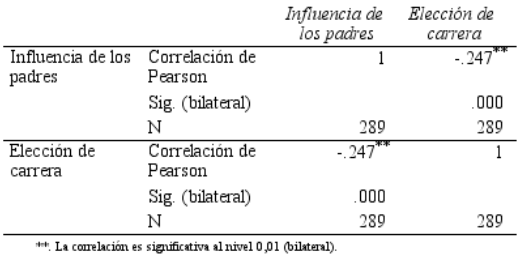
\includegraphics{padresEleccion}
		\caption{Correlaci�n entre el grado de influencia de los padres y si los estudiantes escogieron su carrera}
		\label{fig:padresEleccion}
	\end{center}
\end{table}


